% This template was partially made with assistance from Microsoft Co-pilot

% ------------------------------------------------------------------
% CAPSTONE SOFTWARE REQUIREMENTS SPECIFICATION (SRS)

% 
% This template is inspired by IEEE 29148 but simplified for use in 
% a senior software engineering capstone project. 
% 
% The goal is not to maximize document length. 
% The goal is to produce a clear, testable, and traceable set of 
% requirements that can guide design, implementation, and testing. 
% 
% Recommended workflow: 
% Stakeholder Requirements 
% -> 
% Use Cases 
% -> 
% Functional Requirements 
% -> 
% Acceptance Tests (will be in your VnV plan)
% -> 
% Traceability Matrix (will excluded traceability for tests, that will be in the VnV plan)
% 
% Students should update this document throughout the project. 
% ------------------------------------------------------------------

\documentclass[12pt]{article}

\usepackage{amsmath, mathtools}
\usepackage{amsfonts}
\usepackage{amssymb}
\usepackage{graphicx}
\usepackage{colortbl}
\usepackage{xr}
\usepackage{hyperref}
\usepackage{longtable}
\usepackage{xfrac}
\usepackage{tabularx}
\usepackage{float}
\usepackage{siunitx}
\usepackage{booktabs}
\usepackage{caption}
\usepackage{pdflscape}
\usepackage{afterpage}

\usepackage[round]{natbib}

%\usepackage{refcheck}

\hypersetup{
    bookmarks=true,         % show bookmarks bar?
      colorlinks=true,       % false: boxed links; true: colored links
    linkcolor=red,          % color of internal links (change box color with linkbordercolor)
    citecolor=green,        % color of links to bibliography
    filecolor=magenta,      % color of file links
    urlcolor=cyan           % color of external links
}

\input{../Comments.text}
\input{../Common.text}

% Used so that cross-references have a meaningful prefix

\newcounter{srnum} %Stakeholder Requirement (SR) Number
\newcommand{\srthesrnum}{SR\thesrnum}
\newcommand{\srref}[1]{SR\ref{#1}}

\newcounter{ucnum} %Use Case (UC) Number
\newcommand{\uctheucnum}{UC\theucnum}
\newcommand{\ucref}[1]{UC\ref{#1}}

\newcounter{reqnum} %Functional Requirement (FR) Number
\newcommand{\rthereqnum}{FR\thereqnum}
\newcommand{\rref}[1]{FR\ref{#1}}

\newcounter{nfrnum} %Non-Functional Requirement (NFR) Number
\newcommand{\rthenfrnum}{NFR\thenfrnum}
\newcommand{\nfrref}[1]{NFR\ref{#1}}

\newcounter{lcnum} %Likely Change (LC) Number
\newcommand{\lthelcnum}{LC\thelcnum}
\newcommand{\lcref}[1]{LC\ref{#1}}

\usepackage{fullpage}

\begin{document}

\title{Software Requirements Specification for \progname: subtitle describing software} 
\author{\authname}
\date{\today}
	
\maketitle

~\newpage

\pagenumbering{roman}

\tableofcontents

~\newpage

\section*{Revision History}

\begin{tabularx}{\textwidth}{p{3cm}p{2cm}X}
\toprule {\bf Date} & {\bf Version} & {\bf Notes}\\
\midrule
Date 1 & 1.0 & Notes\\
Date 2 & 1.1 & Notes\\
\bottomrule
\end{tabularx}

~\\
\plt{All capstone SRS documents should have a reflection appendix.}

\newpage

\pagenumbering{arabic}

\plt{This SRS template is based on the IEEE template, with input from co-pilot
  and S. Smith. It will get you started.  You should not modify the section
  headings, without first discussing the change with the course instructor.
  Modification means you are not following the template, which loses some of the
  advantage of a template, especially standardization.}

\plt{Feel free to change the appearance of the report by modifying the LaTeX
  commands.}

\plt{This template document assumes that a single program is being documented.
  If you are documenting a family of models, you should start with a commonality
  analysis.}

\plt{The SRS is not generally written, or read, sequentially.  The SRS is a
  reference document.  It is generally read in an ad hoc order, as the need
  arises.}

\plt{Guiding principles for the SRS document:
\begin{itemize}
\item Do not repeat the same information at the same abstraction level.  If
  information is repeated, the repetition should be at a different abstraction
  level.
\end{itemize}
}

\plt{The template description comments should be disabled before submitting this
  document for grading.}

\plt{You can borrow any wording from the text given in the template.  It is part
  of the template, and not considered an instance of academic integrity.  Of
  course, you need to cite the source of the template.}

\plt{When the documentation is done, it should be possible to trace back to the
  source of every piece of information.  Some information will come from
  external sources, like terminology.}

\plt{An SRS document should have the following qualities: unambiguous,
  consistent, complete, validatable, abstract and traceable.}

\plt{The overall goal of the SRS is that someone can learn,
  understand and verify the captured domain knowledge.  They should not have to
  trust the authors of the SRS on any statements.  They should be able to
  independently verify/derive every statement made.}

% ============================================================== 
\section{Introduction} 
% ==============================================================


\plt{Include a reference to the template this work is based on.  \citet{ISOIECIEEE29148_2018}
justifies the SRS structure and \citet{ISOIECIEEE15288_2023} provides the
broader life-cycle context that underlines modern requirements engineering
practice.}

This document specifies \progname{Magic-8}, a free-to-play, web-based 3D puzzle game built around an 8×8×8 magic cube. 
It states the purpose, users, and project goals: to provide an engaging, navigable magic cube experience in which players complete tasks to practice addition and subtraction in base 8, supported by an introductory tutorial, guided hints, online competitive features, and task-based problem solving. 

The work is based on the provided IEEE SRS template provided in the course {cite} with reference to the ISO/IEC/IEEE 29148:2018 template \citet{ISOIECIEEE29148_2018}, which justifies the SRS structure, 
and ISO/IEC/IEEE 15288:2023, which provides the broader life-cycle context underlying modern requirements engineering practice. Additional sections were added in the form of regulations and guiing protocols, and reasonable inputs & outputs to increase the team's refinement of the project scope and definition.

\subsection{Purpose}

The project is intended to create a game involving an 8x8x8 magic cube that can be navigated by players through task completion to practice addition and subtraction in base 8.
The intent is to solve the lack of engaging resources available for learning and practicing mathematics in non-decimal number bases as alternative bases. Such as base 8, are rarely taught before post-secondary education.

The following sections will outline the scope, functional requirements and the non-functional requirements that the team will adhere to produce a game that is both educative and fun.

\subsection{Scope}

\textbf{In-Scope and functionality}

The project known as \progname will be a free-to-play web game where users will be presented with a 3D visualization of an 8$\times$8$\times$8 magic cube separated into slices.
Users receive a tutorial on addition and subtraction in base eight, a starting cell, and at least 8 tasks that, by solving the problems within, will navigate them through the cube as they move through its layers.
Users will gain points for correctly solving the problems in a task; these points will be tied to a user's personal account.

\textbf{Intended users}

Magic-8 primarily appeals to recreational math enjoyers who would enjoy a challenge while practicing a different base, and high school students and their teachers who gain a way to engagingly experience an unfamiliar base.
The goal is to create a system that can not only be used as a fun way to improve one's skill in addition and subtraction in bases but would also act as a ready-made introductory classroom tool for engaging students,
an experience that is helpful for aspiring STEM students due to how important base 8 and working with new number bases is in systems such as Unix, the C programming language, etc., with Magic-8 serving as an early introduction. As such,
the improved interest in numeracy stemming from a broader appreciation for alternative number bases benefits all those who would appreciate the greater interest, such as
post-secondary STEM professors, educational technology platforms, and society as a whole.

\textbf{Out of Scope}

The tool is aimed at being fun and educational; it is not intended to replace a curriculum or full octal tutorial; it is strictly web-based with no plans for mobile or offline development.
It supports octal only (no other bases, no 2D squares, no 4D tesseracts, no alternative rulesets, no automatic cube generation, no player puzzle generation, no decimal mode, although these may be considered as stretch goals after project completion).
Cubes of order other than 8 and 16 are excluded because they do not satisfy all 13 lines.

\textbf{Explicit assumptions}

The project assumes the following as true for the success of the project:
\begin{itemize}
\item A valid order 8 magic cube is available.
\item New valid cubes can be created be it algorithmically or through rotation of initial cube.
\item A user will not be able to memorize the positions of the 512 cells that make up the cube to bypass task interaction.
\item Users have browser capable devices and internet access.
\item Users posses basic numeracy.
\item The chosen implementation software's open source licenses are compatible with the distribution method.
\item Tasks are all solveable and their problems can be accurately conveyed to intended users.
\item Users are willing to engage with an octal system.
\end{itemize}

\subsection{Stakeholders}
A stakeholder for the project is defined as any independent party with an interest in the sucess of the game or is affected by it. The team will categorize 
stakeholders following the SRS IEEE template however due to our team acting as the development team the development team category will not apply.

\begin{itemize}
\item \textbf{Customer:}
      The game is free to play; however, technological educational websites who may choose to host the website to increase their catalog. The aim is also for high school teachers to adopt the game as a way of maintaining students' attention
      in fun and educational activities that are still classroom appropriate.
\item \textbf{End Users:} 
      The end users include the recreational math enthusiasts who play the game for intellectual stimulation and the novelty of magic cube mathematics; they may already be familiar with octal, but their main goal is entertainment over education. 
      Another primary end user are the high school students who play the game to practice basic octal in a way that they find engaging.
\item \textbf{Project Sponsor:}
      The capstone supervisor endorses and provides the context and the initial goals which the project team should meet; their involvement means the project needs to meet its stated goals within the capstone timeline
      and demonstrate its recreational value as can be seen from their history in proposing recreational math games. The supervisor also provides institutional insight that guides how the project is specified and implemented, with suggestions
      on the ways cubes can be generated, presented to the user, and how difficulty and tasks should be addressed.
\item \textbf{Administrators:}
      The administrators for this project would be in charge of managing the online components of Magic-8 such as the user account and login information and are concerned with ensuring the privacy and integrity of the user data.
      In a similar vein, the regulatory and ethics bodies that set rules for data minimization and privacy protection policies are concerned with the game meeting all their related policies.
\item \textbf{Society:}
      Society in this context refers to the general public; one of the game's goals is to educate and breed interest in society for mathematics. This is intended to increase the numeracy of the general public and increase interest in programs such as mathematics and engineering.
      As it is intended to reach the general public, there is also interest from the families of users in the game being free, safe, private, and inclusive to those from any background and conscious of the health issues that might be faced by the users,
      requiring careful thought into how the visuals, inputs, and outputs are handled to make them non-safety critical or triggering in any way. The product will likely be used by more vulnerable members of society such as teenagers, and thus care must be given to ensuring their 
      information and safety are not compromised from their gaming experience.
\end{itemize}


\subsection{Regulations and guiding protocols}
The project must satisfy all the foloowing rules and regulations: 

\begin{longtable}{p{0.25\textwidth} p{0.65\textwidth}}
\toprule
Standard / Protocol & Description\\
\midrule
\endfirsthead
\toprule
Standard / Protocol & Description\\
\midrule
\endhead
\endlastfoot
ISO/IEC/IEEE 29148:2018 & International standard defining the structure and content of requirements specifications, used to justify the organization of this SRS. \\
ISO/IEC/IEEE 15288:2023 & International standard describing software and systems life-cycle processes, providing the broader engineering context for requirements practice. \\
WCAG 2.1 Level AA & Web Content Accessibility Guidelines defining accessibility requirements for web content; the game targets Level AA for keyboard navigation, contrast, and text resizing. \\
W3C WebAssembly & World Wide Web Consortium standard for portable binary code executed in browsers; the game is packaged via pygbag to run as a WebAssembly module. \\
W3C HTML5 & World Wide Web Consortium standard for web page structure and browser interaction; the game interface must conform to it. \\
GDPR & General Data Protection Regulation governing the processing and protection of personal data for users in the European Union. \\
PIPEDA & Personal Information Protection and Electronic Documents Act governing personal data handling for users in Canada. \\
COPPA & Children's Online Privacy Protection Act governing data collection from users under 13; applies if the game is made available to children below that age. \\
FERPA & Family Educational Rights and Privacy Act governing student education records; applies if the game is integrated into formal classroom settings. \\
Open-source licenses & Licensing terms of libraries such as pygame-ce, pygbag, pylint, pytest, and mypy; the game must comply with all dependency licenses. \\
\bottomrule
\caption{Regulations and Guiding Protocols} \label{tab:RegulationsAndProtocols}
\end{longtable}

\subsection{Reasonable Inputs and Outputs}

The following outlines some of the projects expected user inputs:

\begin{longtable}{p{0.25\textwidth} p{0.65\textwidth}}
\toprule
Input & Description\\
\midrule
\endfirsthead
\toprule
Input & Description\\
\midrule
\endhead
\endlastfoot
3D navigation commands & Rotation, zoom, and movement through cube layers via keyboard or mouse. \\
Voxel selection & Selecting a specific voxel number within the cube. \\
Answer submission & Submitting a selected voxel or value as the answer to the current task. \\
Tutorial interactions & Advancing through, replaying, or skipping the tutorial. \\
Account credentials & Username and password for account creation and login. \\
Round start & Player begins a new round, triggering task generation. \\
Database state & Stored accounts and statistics, retrieved from local or online databases. \\
Authentication responses & Responses from third-party identity providers, if integrated. \\
Asset and configuration files & Game assets, cube visuals, and configuration data loaded at startup. \\
\bottomrule
\caption{Project Inputs} \label{tab:ProjectInputs}
\end{longtable}

The following outlines some of the projects expected user inputs:

\begin{longtable}{p{0.25\textwidth} p{0.65\textwidth}}
\toprule
Output & Description\\
\midrule
\endfirsthead
\toprule
Output & Description\\
\midrule
\endhead
\endlastfoot
3D cube rendering & Visual display of the 8$\times$8$\times$8 magic cube with visible and hidden voxels. \\
Slice and voxel highlighting & Visual differentiation of slices, selected voxels, and active lines. \\
Task progress display & Current task, progress within the round, and remaining tasks. \\
Correct/incorrect indication & Clear feedback on whether an answer was correct or incorrect. \\
Error explanations & Explanation of mistakes users make while playing. \\
Score and statistics display & Points earned, times, accuracy, and other gameplay statistics. \\
Tutorial content & Interactive instructional content for learning to play and for octal basics. \\
Account confirmations & Confirmation of account creation and login. \\
Local database updates & Stored accounts, statistics, and settings persisted on the user's device. \\
Online database updates & Synchronized accounts and game statistics on the server. \\
\bottomrule
\caption{Project Outputs} \label{tab:ProjectOutputs}
\end{longtable}

\subsection{Definitions and Acronyms}

This section provides the meaning of the different words and phrases used
in the domain of the problem.

\begin{longtable}{p{0.25\textwidth} p{0.65\textwidth}}
\toprule
Term & Definition\\
\midrule
Base 8 & A number system using the digits 0 to 7 where the value for each digit in decimal can be found by multiplying by 8 to the power of n where n represents the number of positions from the right. \\
Octal & Another name for base 8. \\
Magic square & A square array of positive integers where the sum of each individual row, column, or main diagonal is the same.\\
Magic cube & The 3-dimensional equivalent of a magic square where the sums of each row, column, pillar, main diagonal, or triagonal is the same. \\
Magic constant & The fixed sum obtained when doing sums in any row, column, or main diagonal in a magic square. \\
Most perfect magic cube & A magic cube where all rows, columns, pillars, diagonals, triagonals, and broken space diagonals add up to the magic constant. \\
Triagonal & A line or set of cells connecting two opposite vertices through the interior of a cube and hence moves across all three axes. \\
Broken space diagonal & A diagonal that wraps around the cube's boundaries.\\
Voxel & A single 3D cell within the magic cube. \\
Slice & A 2D display providing all the voxels within a certain cross section of the magic cube.\\
Round & A single playthrough of the game consisting of 8 sequential tasks. \\
Starter & The initial randomly chosen visible voxel that acts as a starting point for the player to start solving tasks.\\
\bottomrule
\caption{Definitions and Acronyms} \label{tab:DefinitionsAndAcronyms}
\end{longtable}

\subsection{Characteristics of Intended Reader} \label{sec_IntendedReader}

The intended readers of this document are expected to be able to read, review, maintain, or implement the SRS. 
As such, they are expected to have knowledge equivalent to the final year of a software engineering student or a student of an equivalent degree.
This includes an intermediate level of experience with a programming language such as Python, a beginner level understanding of 3D graphics, game development, WebAssembly, and CI/CD.

% ============================================================== 
\section{System Overview}

This section provides general information about the system.  It identifies the
problem, the vision, and the interfaces between the system and its environment.
This section also describes user characteristics and lists the system
constraints.

%\plt{The purpose of this section is to provide general information about the
  %system so that the specific requirements in the later sections will be easier to
  %understand. The general system description section is designed to be
  %changeable independent of changes to the functional requirements documented in
  %the specific system description. The general system description provides a
  %context for a family of related models.  The general description can stay the
  %same, while specific details are changed between family members.}

\subsection{Problem Statement}

%\plt{Current situation, problem, impact, desired improvement.  You will likely borrow some text from your problem description document.}

Magic cubes provide an opportunity to explore numerical patterns and mathematical 
relationships in 3-dimensions. However, understanding these structures can become
challenging due to limited sources as well as having to use static 2D images to understand
a 3D pattern.

The goal of this project is to create a recreational mathematics game that allows those interested
in these magic cubes as well as non standard number bases such as base 8 to further their understanding.
This is planned to be a web-based game in which users will be able to complete certain challenges on a 3d
representation of an 8x8x8 magic cube using base 8 mathematics to find patterns associated with a magic cube.
This will include adding values to certain sections of the cube to complete patterns of magic cubes moving through
8 stages of difficulty while continuing to learn about these mathematical structures.

\subsection{Product Vision}

%\plt{A clear and concise statement of the product's purpose and goals.}

%\plt{The goal statements are functional and nonfunctional objectives that system
  %under consideration should achieve. Goals provide criteria for sufficient
  %completeness of a requirements specification and for requirements pertinence.
  %Goals will be refined by requirements.  The goals are written abstractly, with
  %a minimal amount of technical language.  They should be understandable by
  %non-domain experts.}

%\plt{You will likely borrow from your goal statements in your problem
%description document.}

The vision for Magic-8 is to provide an accessible and engaging recreational mathematics application
to allow interested users to further their understanding of non base 10 number systems as well as mathematical
patterns found in objects such as magic cubes. The system will allow for simple interaction with the magic cube
to allow users to see its many different views as well as help educate them in the patterns they will be using
throughout the challenges.

This will be able to operate on supported desktop and laptop web browsers and will provide some account-based storage to
track the users performance and rank them on a leaderboard. The system is planned to focus on maintainable and modular system
design to potentially allow for different number bases in the future as well as ease of use for the users of the application.
  
\subsection{System Context}

%\plt{Include users, external systems, APIs, databases, and third-party services.}

%\plt{Your system context will include a figure that shows the abstract view of
  %the software.  In some cases the diagram will show other external
  %entities, besides the user.  For instance, when the software product is a
  %library, the user will be another software program, not an actual end user.
  %If there are system constraints that the software must work with external
  %libraries, these libraries can also be shown on the System Context diagram.
  %They should only be named with a specific library name if this is required by
  %the system constraint.}

\begin{figure}[h!]
\begin{center}
 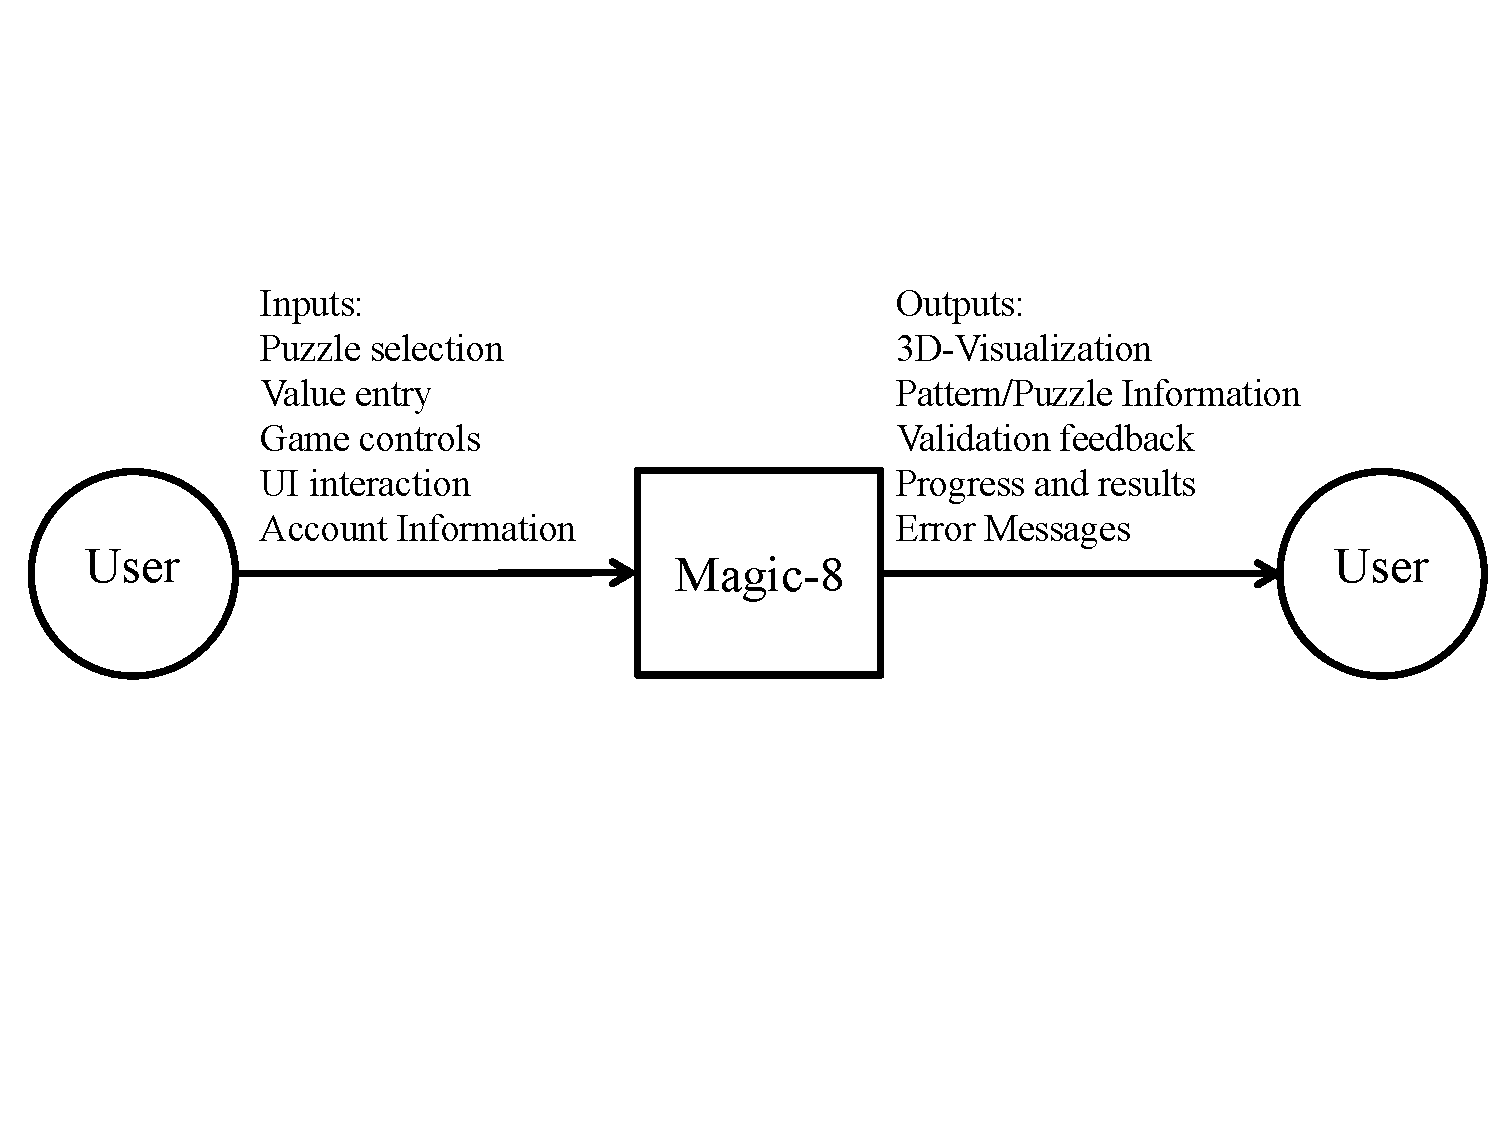
\includegraphics[width=0.6\textwidth]{SystemContextFigure}
\caption{System Context}
\label{Fig_SystemContext} 
\end{center}
\end{figure}

%\plt{For each of the entities in the system context diagram its responsibilities
  %should be listed.  Whenever possible the system should check for data quality,
  %but for some cases the user will need to assume that responsibility.  The list
  %of responsibilities should be about the inputs and outputs only, and they
  %should be abstract.  Details should not be presented here.  However, the
  %information should not be so abstract as to just say ``inputs'' and
  %``outputs''.  A summarizing phrase can be used to characterize the inputs.
  %For instance, saying ``material properties'' provides some information, but it
  %stays away from the detail of listing every required properties.}

\begin{itemize}
\item User Responsibilities:
\begin{itemize}
\item Provide the information required for supported account
  operations.
\item Select puzzles or activities and provide numerical
  inputs through the interface.
\item Use the available controls to manipulate the cube, select
  cells, and edit cell values.
\item Review validation messages and feedback provided by
  the application.
\end{itemize}
\item \progname{} Responsibilities:
\begin{itemize}
\item Validate user inputs and identify invalid or
  unsupported values.
\item Process supported cube interactions and maintain
  the current puzzle state.
\item Present the cube and associated numerical information
  in the user interface.
\item Provide feedback about input validation and the
  outcomes of supported operations.
\item Communicate with the online service to authenticate
  users and save or retrieve designated user data.
\item Inform users when account or storage operations fail
  or cannot be completed.
\end{itemize}
\item Web Browser Responsibilities:
\begin{itemize}
\item Execute the delivered application and provide the
  environment in which its interface is displayed.
\item Render the two-dimensional interface and
  three-dimensional cube visualization.
\item Relay user interactions to the application.
\end{itemize}
\end{itemize}

%\plt{Identify in what context the software will typically be used.  Is it for
%exploration? education? engineering work? scientific work?. Identify whether it
%will be used for mission-critical or safety-critical applications.} 

%\plt{This additional context information is needed to determine how much effort
%should be devoted to the rationale section.  If the application is
%safety-critical, the bar is higher.  This is currently less structured, but
%analogous to, the idea to the Automotive Safety Integrity Levels (ASILs) that
%McSCert uses in their automotive hazard analyses.}

Magic-8 is intended for recreational and educational exploration. This means it will
not be operating in a highly safety or mission-critical enviornment. The application
provides a simple way to interact with slighlty more obscure mathematical ideas rather
than any critical operations.

\subsection{User Characteristics} \label{SecUserCharacteristics}

%\plt{This section summarizes the knowledge/skills expected of the user.
  %Measuring usability, which is often a required non-function requirement,
  %requires knowledge of a typical user.  As mentioned above, the user is a
  %different role from the ``intended reader,'' as given in
  %Section~\ref{sec_IntendedReader}.  As in Section~\ref{sec_IntendedReader}, the
  %user characteristics should be specific an unambiguous.  For instance, ``The
  %end user of \progname{} should have an understanding of undergraduate Level 1
  %Calculus and Physics.''}

The intended users are individuals who are interested in recreational mathematics,
numerical puzzles and structures, and non standard number bases. Users may range from
beginners who may have just started learning base 8 and never encountered magic cubes
or vice versa, to experienced mathematical enthusiasts interested in trying a new challenge.

Users are expected to have basic computer skills, including the ability to navigate a web browser,
use pointer-based controls, and enter numerical values. No programming knowledge is required for use.
Only basic mathematic understanding of addition and subtraction is expected as the application can help 
to teach the subjects it covers.

\subsection{System Constraints}

%\plt{System constraints differ from other type of requirements because they
  %limit the developers' options in the system design and they identify how the
  %eventual system must fit into the world. This is the only place in the SRS
  %where design decisions can be specified.  That is, the quality requirement for
  %abstraction is relaxed here.  However, system constraints should only be
  %included if they are truly required.}

%\plt{This is where you would mention platform constrains, and licensing
%restrictions.}

Magic-8 shall be designed to run within desktop and laptop web browsers without requiring an installation.
The functionality will initially be developed in python as well as supported python libraries such as pygame.
It will then be translated into webassembly code for execution in browser. This means that all python code must be
translatable with the chosen tool into webassembly including anything used for the user interface of the application.

The system shall also support online account functionality, requiring network communication with the selected 
service for remote data operations. The specific service, supported web browsers, and rendering technologies 
are yet to be established. This will happen as implementation decisions are finalized.

% ============================================================== 
\section{Stakeholder Requirements}

\plt{Technology-independent requirements.  These come from statements made by
the stakeholders.  You will find these through interviews and surveys.  They are
often expressed in natural language.  They are not necessarily testable, but
they should be verifiable.}

\plt{The stakeholder requirements are numbered so that you can have traceability to other parts of your document.}

\noindent \begin{itemize}

\item[SR\refstepcounter{srnum}\thesrnum \label{SR_Label1}] TODO

\item[SR\refstepcounter{srnum}\thesrnum \label{SR_Label2}] TODO

\item[SR\refstepcounter{srnum}\thesrnum \label{SR_Label3}] TODO

\end{itemize}

\plt{You should give your SRs meaningful labels, so that you can refer to them
in other parts of the SRS.  The label names should be meaningful mnemonics, not
numbers.}

% ============================================================== 
\section{User Personas}
\plt{Create 2-5 realistic personas.
  Personas are fictional characters that represent the different user types that
  might use your software.  They are used to help understand the users'
  needs, experiences, behaviors and goals.  They are not real people, but they
  should be based on real data collected from user research.}

\subsection{Persona 1}
\begin{itemize}
\item Name:
\item Description:
\item Goals:
\item Frustrations:
\item Technical Ability:
\end{itemize}

\subsection{Persona 2}
\begin{itemize}
\item Name:
\item Description:
\item Goals:
\item Frustrations:
\item Technical Ability:
\end{itemize}

% ============================================================== 
\section{Use Cases}
\plt{Use cases are a way to describe the interactions between users and the system.
  They are typically written in natural language and describe the steps that a
  user takes to achieve a specific goal.  Use cases can be used to identify
  functional requirements and to create test cases.}  
\plt{Typically 8-15 substantial use cases.}

\refstepcounter{ucnum} \label{UC_Label1}
\subsection{\ucref{UC_Label1}: Example Use Case}

\textbf{Primary Actor}

TODO

\textbf{Preconditions}
\begin{itemize}
\item TODO
\end{itemize}

\textbf{Main Success Scenario}
\begin{enumerate}
\item TODO
\item TODO
\item TODO
\end{enumerate}

\textbf{Alternative Flows}
\begin{itemize}
\item TODO
\end{itemize}

\textbf{Postconditions}
\begin{itemize}
\item TODO
\end{itemize}

% ============================================================== 
\section{Functional Requirements}
\plt{Functional requirements describe what the system should do.  They are typically
expressed as a set of conditions or capabilities that the system must have.  These
requirements are usually derived from the stakeholder requirements and use cases.}

\plt{Use SHALL statements. Requirements must be atomic, testable, and traceable.}

\noindent \begin{itemize}

\item[FR\refstepcounter{reqnum}\thereqnum \label{FR_Label1}:] The system shall ...

\item[FR\refstepcounter{reqnum}\thereqnum \label{FR_Label2}:] The system shall ...

\item[FR\refstepcounter{reqnum}\thereqnum \label{FR_Label3}:] The system shall ...

\end{itemize}

\plt{The requirements are given labels so that they can be referenced in other
parts of the SRS.  The label names should be meaningful mnemonics, not numbers.}

% ============================================================== 
\section{Data Requirements}

\plt{The Data Requirements section describes what information the system must manage.
  It includes the major data entities, their attributes, and the relationships
  between them.  It also includes a data dictionary that defines the meaning of
  each attribute.}

\subsection{Major Data Entities}

\plt{What information must exist for the system to accomplish its goals?}

\plt{For each entity, provide a short explanation.}

\begin{itemize}
\item User
\item Song
\item Session
\item Report
\end{itemize}

\subsection{Data Dictionary}

\plt{For each entity, define all important attributes.}

\begin{longtable}{p{0.20\textwidth} p{0.20\textwidth} p{0.45\textwidth}}
\toprule
Attribute & Type & Description\\
\midrule
user\_id & UUID & Unique identifier\\
email & String & User email address\\
\bottomrule
\caption{Data Dictionary} \label{tab:DataDictionary}
\end{longtable}

\subsection{Privacy and Data Retention}

\plt{Discuss storage, retention, deletion, privacy controls,
 consent, encryption, and compliance requirements.}

TODO

% ============================================================== 
\section{Non-Functional Requirements}

%\plt{You may have to add other NFRs.}

%\plt{List your nonfunctional requirements.  You may consider using a fit
  %criterion to make them verifiable.}

%\plt{The goal is for the nonfunctional requirements to be unambiguous, abstract
  %and verifiable.  This isn't easy to show succinctly, so a good strategy may be
%to give a ``high level'' view of the requirement, but allow for the details to
%be covered in the Verification and Validation document.}

%\plt{An absolute requirement on a quality of the system is rarely needed.  For
  %instance, an accuracy of 0.0101 \% is likely fine, even if the requirement is
  %for 0.01 \% accuracy.  Therefore, the emphasis will often be more on
  %describing now well the quality is achieved, through experimentation, and
  %possibly theory, rather than meeting some bar that was defined a priori.}

%\plt{You do not need an entry for correctness in your NFRs.  The purpose of the
  %SRS is to record the requirements that need to be satisfied for correctness.
  %Any statement of correctness would just be redundant. Rather than discuss
  %correctness, you can characterize how far away from the correct (true)
  %solution you are allowed to be.  This is discussed under accuracy.}

\noindent
\begin{itemize}

\item[NFR\refstepcounter{nfrnum}\thenfrnum
\label{NFR_Performance}:]
\textbf{Performance}

Under the defined reference test enviornment, the system shall
update the visible cube orientation within 100 milliseconds of
a supported rotation input. The system shall also reflect an
accepted cell-value edit in the relevant two-dimensional and
three-dimensional views within 100 milliseconds.

\item[NFR\refstepcounter{nfrnum}\thenfrnum
\label{NFR_Usability}:]
\textbf{Usability}

The majority of participants (most likely at least 80\%) in a usability evaluation shall
complete each of the following tasks without external assistance:
opening a puzzle, manipulating the 3D visual cube, selecting a cell, 
and editing a cell value.

\item[NFR\refstepcounter{nfrnum}\thenfrnum
\label{NFR_Maintainability}:]
\textbf{Maintainability}

The mathematical logic, user-interface logic, three-dimensional
visualization logic, and online storage interactions shall be
organized into identifiable components with documented
responsibilities. This will be measured with the fit criterion:
Automated tests for the core mathematical operations shall 
be executable independently of the user interface.

\item[NFR\refstepcounter{nfrnum}\thenfrnum
\label{NFR_Portability}:]
\textbf{Portability}

The system shall execute in each desktop and laptop web browser
that it is stated to support without requiring users to install Python 
or a standalone desktop application. The core test suite shall pass on each 
supported browser.

\item[NFR\refstepcounter{nfrnum}\thenfrnum
\label{NFR_Reliability}:]
\textbf{Reliability}

The system shall maintain a valid in-memory puzzle state following
supported cube modifications, cell selections, and valid cell-value
edits. Invalid user inputs shall be handled without terminating
the application or leaving the puzzle state invalid. If an online 
operation fails, the system shall inform the user
and shall not indicate that the operation succeeded.

\item[NFR\refstepcounter{nfrnum}\thenfrnum
\label{NFR_Security}:]
\textbf{Security and Privacy}

All network communication involving account credentials or
user data shall use HTTPS with valid TLS. The system shall prevent
authenticated users from accessing other users' private stored
data through its supported interfaces and operations.
Application-controlled persistent storage shall not store
authentication secrets in plaintext. The application shall collect
only the personal information necessary for its implemented functionality.

\item[NFR\refstepcounter{nfrnum}\thenfrnum
\label{NFR_Accessibility}:]
\textbf{Accessibility}

All essential puzzle controls shall be operable using a keyboard
without requiring pointer interaction. Essential interface text
and controls shall be clearly visible with high contrast (3:1). 
The system shall provide a two-dimensional method of viewing
and editing cell values so that essential puzzle
operations do not depend exclusively on manipulating the
three-dimensional visualization.

\end{itemize}

% ============================================================== 
\section{AI and Machine Learning Requirements}

\plt{Refer to
\href{https://gitlab.cas.mcmaster.ca/courses/capstone/-/blob/main/Lectures/Lxx_DrMosserGuestLecture/2026_09_Capstone.pdf?ref_type=heads}{Dr.
Mosser's guest lecture} on AI requirements.}

\plt{Include only when applicable.}

\subsection{Model Inputs}

TODO

\subsection{Model Outputs}

TODO

\subsection{Evaluation Metrics}

\plt{Accuracy, Precision, Recall, F1, BLEU, WER, etc.}

TODO

\subsection{Known Limitations}

\plt{Explicitly document expected failure modes.}

TODO

% ============================================================== 
\section{Requirements Traceability Matrices}

\plt{The Requirements Traceability Matrix (RTM) is a table that shows the
relationship between different types of requirements. It is used to ensure that
all requirements are traceable and that no requirements are missed. The typical
flow is: Stakeholder Need -> Use Case -> Requirement}

\plt{There is also a traceability matrix between functional and nonfunctional
  requirements. The purpose of some FRs is to satisfy NFRs.  Therefore, it is
  important to show the relationship between the two.}

\plt{Further traceability to test cases and modules will be given in other
documents.}

\begin{longtable}{p{0.15\textwidth} p{0.15\textwidth} p{0.20\textwidth} p{0.20\textwidth}}

\toprule
Stakeholder Req & Use Case & Functional Req \\
\midrule
\srref{SR_Label1} & \ucref{UC_Label1} & \rref{FR_Label1} \\
\bottomrule

\caption{Traceability Between Stakeholder Requirements, Use Cases, and
Functional Requirements} \label{tab:SR2UC2FRtm}
\end{longtable}

\begin{longtable}{p{0.20\textwidth} p{0.20\textwidth}}

\toprule
Functional Req & Nonfunctional Req \\
\midrule
\rref{FR_Label1} & \nfrref{NFR_Accuracy} \\
\bottomrule
\caption{Traceability Between Functional and Nonfunctional Requirements}
\label{tab:FR2Rtm}

\end{longtable}

% ============================================================== 

\section{Rationale}

\plt{Provide a rationale for the decisions made in the documentation.  Rationale
should be provided for scope decisions, functional requirements, nonfunctioanl
requirements, data requirements, and AI requirements.  You don't need a
rationale for everything, ust the major decisions that are not obvious.  You
should have traceability to the entities in the document that you are
referencing.}

\section{Likely Changes}    

\noindent \begin{itemize}

\item[LC\refstepcounter{lcnum}\thelcnum\label{LC_meaningfulLabel}:] \plt{Give
    the likely changes, with traceability to the entity that is likely to change.}

\end{itemize}

\section{Unlikely Changes}    

\noindent \begin{itemize}

\item[LC\refstepcounter{lcnum}\thelcnum\label{LC_meaningfulLabel}:] \plt{Give
    the unlikely changes.  The design can assume that the changes listed will
    not occur.}

\end{itemize}

\newpage{}

\section{Appendices}

\subsection{Appendix A: Additional Materials}

TODO

\subsection{Appendix B: Development Plan}

\plt{This section is optional.  It is used to explain the plan for developing
  the software.  In particular, this section gives a list of the order in which
  the requirements will be implemented.  In the context of a course  this is
  where you can indicate which requirements will be implemented as part of the
  course, and which will be ``faked'' as future work.  This section can be
  organized as a prioritized list of requirements, or it could show the
  requirements that will be implemented for ``phase 1'', ``phase 2'', etc.}

\subsection{Appendix C: Values of Auxiliary Constants}

\plt{Show the values of the symbolic parameters introduced in the report.}

\plt{The definition of the requirements will likely call for SYMBOLIC\_CONSTANTS.
Their values are defined in this section for easy maintenance.}

\plt{The value of FRACTION, for the Maintainability NFR would be given here.}

TODO

\subsection{Appendix D: Generative AI Disclosure}

\plt{Provide full transparency on how generative AI was used in the creation of
  this document.  This includes any text, figures, or tables that were generated
  by AI.  If any skills were created for AI agents to review the documentation,
  those should be disclosed here.}

\subsection{Appendix E: Reflection}

\plt{This isn't part of the SRS, but it is part of the course.}

The information in this section will be used to evaluate the team members on the
graduate attribute of Lifelong Learning.  

\input{../Reflection.text}

\input{../SRS_Reflection.text}

\newpage

\bibliographystyle {plainnat}
\bibliography {../../refs/References}

\newpage


\end{document}